\externaldocument{tech_eclipse_text}

\subsection{Results \label{results}}
The program does a good job of recovering the input brightness values and matching the light curves. The level of noise has some effect on the reproduction of the brightness values, but clear trends can still be seen even with simulated 14th magnitude noise. One important thing to note is that the program does not recover the correct brightness values every time, but does a good job when averaged over many windows. This means that the results are better interpreted as long term trends than as exactly correct in every window. For the synthetic light curves, starspot evolution was not introduced. However, in real systems starspot evolution would exist. This means that our program can give information about overall trends in starspot evolution, but it cannot be trusted to give the exact brightness values of a region for any given time step. 

In all cases, the light curve fits look good for synthetic curves and real data alike. The fit of the light curve is good irrespective of noise level in the synthetic curve.

To visualize the brightness values, we use Figures~\ref{stripe_plot} and~\ref{box_plot}. The value on the far right is the input value for the synthetic light curves. The y-axis in these images represents longitude along the stellar surface.

\begin{figure}[h]
	\centering
	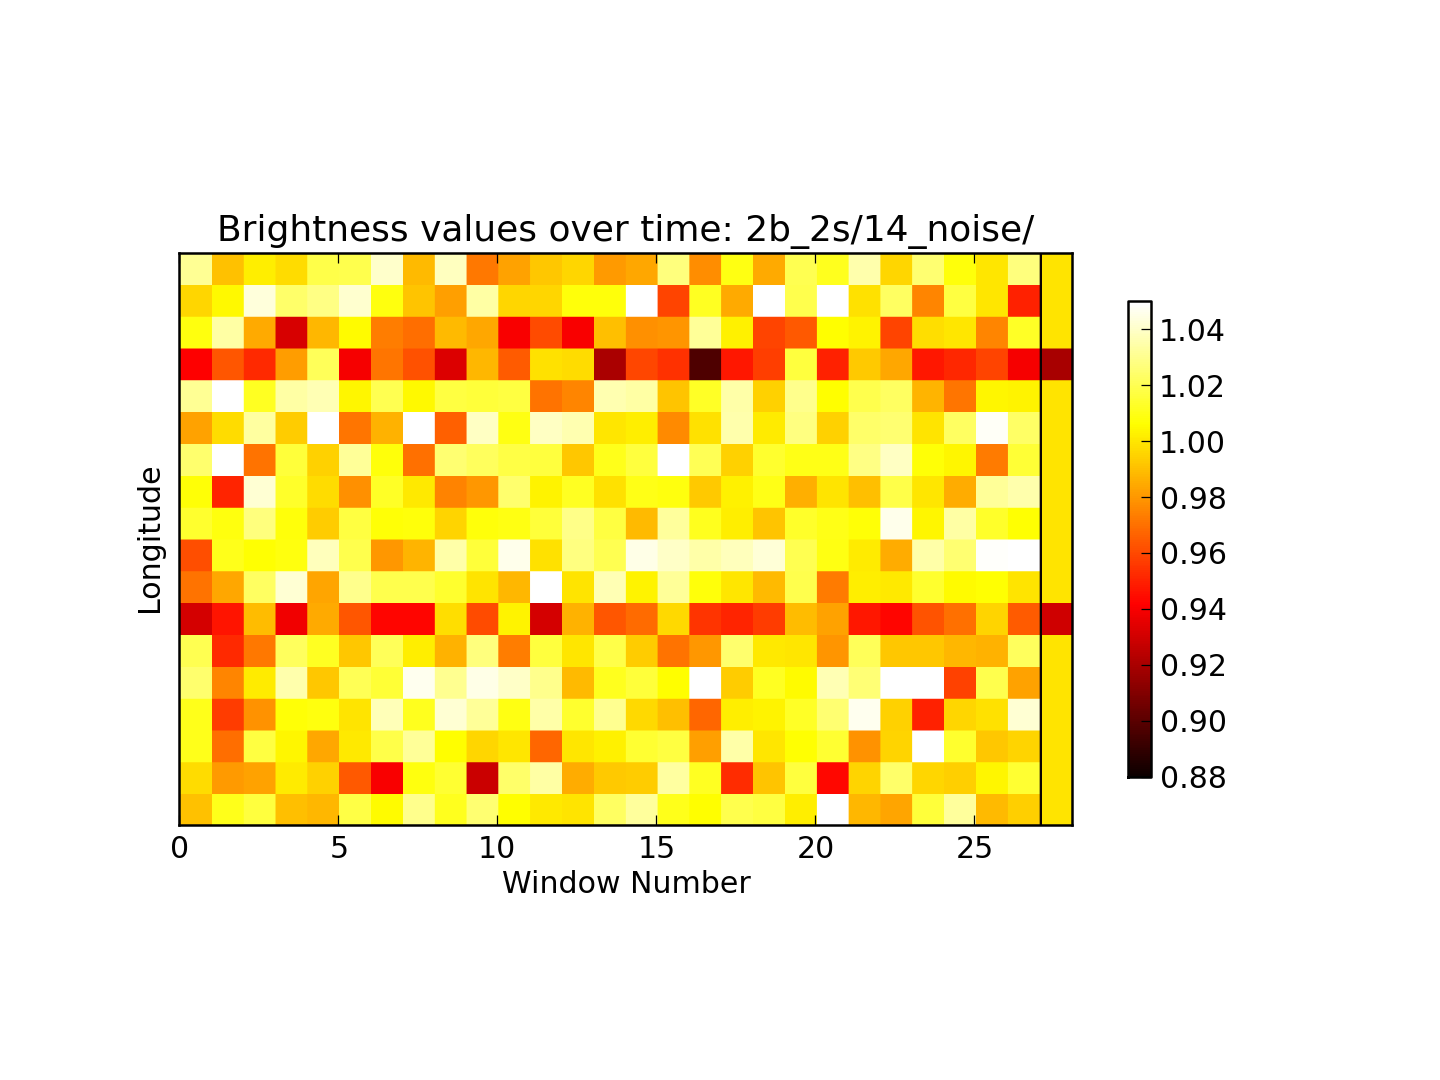
\includegraphics[width=.5\textwidth]{images/2b_2s/14_noise/box_plot.png}
	\caption{Recovered stripe brightness plot versus window number. The color bar (right) shows the relative brightness value relations to the color scale.}
	\label{box_plot}
\end{figure}
\begin{figure}[h]
	\centering
	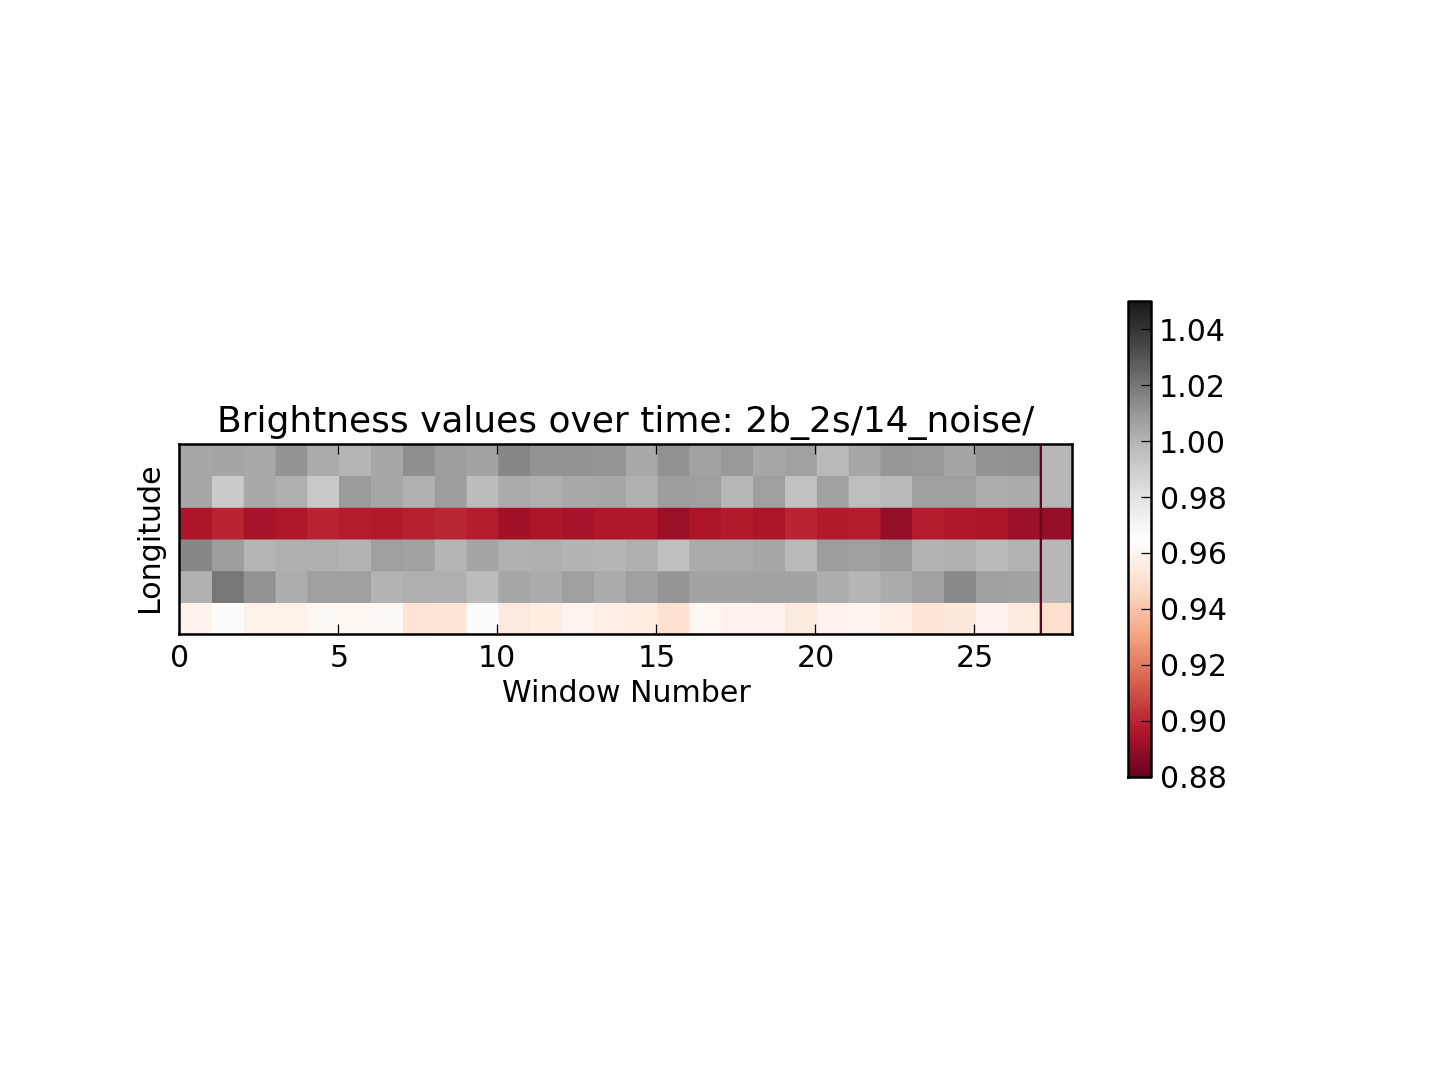
\includegraphics[width=.5\textwidth]{images/2b_2s/14_noise/stripe_plot.png}
	\caption{Recovered stripe brightness plot versus window number. The color bar (right) shows the relative brightness value relations to the color scale.}
	\label{stripe_plot}
\end{figure}
\begin{figure}[h]
	\centering
	\includegraphics[width=.5\textwidth]{images/1b/14_noise/stripe_plot.png}
	\caption{Recovered stripe brightness plot versus window number. The color bar (right) shows the relative brightness value relations to the color scale.}
	\label{stripe_plot14}
\end{figure}
\begin{figure}[h]
	\centering
	\includegraphics[width=.5\textwidth]{images/1b/noise/stripe_plot.png}
	\caption{Recovered stripe brightness plot versus window number. The color bar (right) shows the relative brightness value relations to the color scale.}
	\label{stripe_plot12}
\end{figure}
\begin{figure}[h]
	\centering
	\includegraphics[width=.5\textwidth]{images/1b/no_noise/stripe_plot.png}
	\caption{Recovered stripe brightness plot versus window number. The color bar (right) shows the relative brightness value relations to the color scale.}
	\label{stripe_plot}
\end{figure}
\begin{figure}[h]
	\centering
	\includegraphics[width=.5\textwidth]{images/1b/14_noise/box_plot.png}
	\caption{Recovered box brightness plot versus window number. The color bar (right) shows the relative brightness value relations to the color scale.}
	\label{box_plot14}
\end{figure}
\begin{figure}[h]
	\centering
	\includegraphics[width=.5\textwidth]{images/1b/noise/box_plot.png}
	\caption{Recovered box brightness plot versus window number. The color bar (right) shows the relative brightness value relations to the color scale.}
	\label{box_plot12}
\end{figure}
\begin{figure}[h]
	\centering
	\includegraphics[width=.5\textwidth]{images/1b/no_noise/box_plot.png}
	\caption{Recovered box brightness plot versus window number. The color bar (right) shows the relative brightness value relations to the color scale.}
	\label{box_plot}
\end{figure}
\begin{figure}[h]
	\centering
	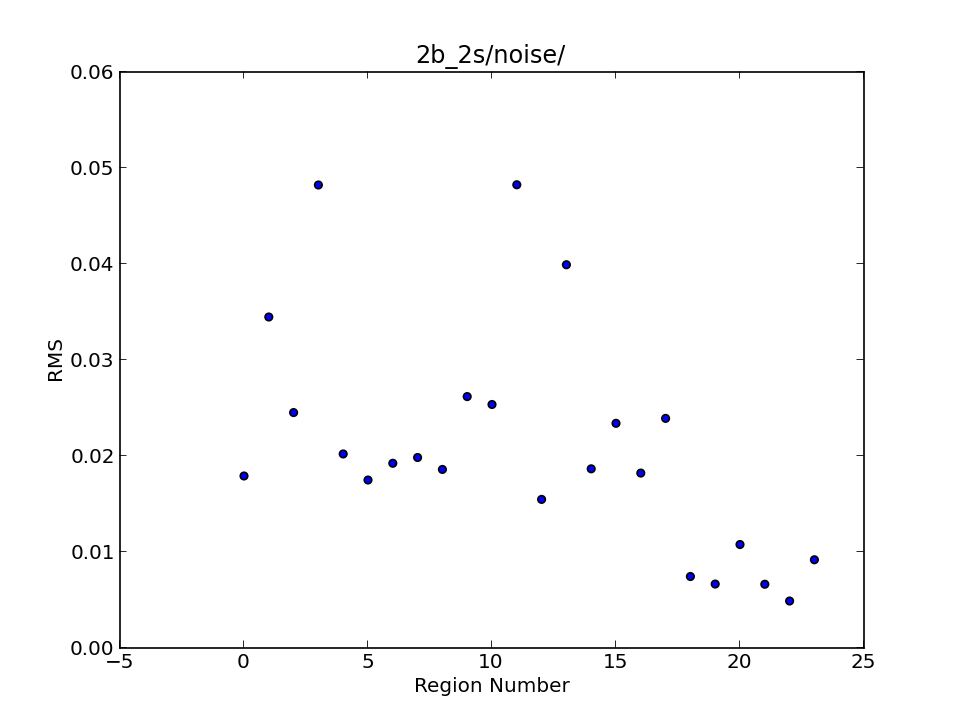
\includegraphics[width=.5\textwidth]{images/1b/14_noise/rms_over_time.png}
	\caption{RMS between the brightness values used to produce the synthetic curves and the brightness values recovered by the Amoeba Algorithm.}
	\label{rms14}
\end{figure}
\begin{figure}[h]
	\centering
	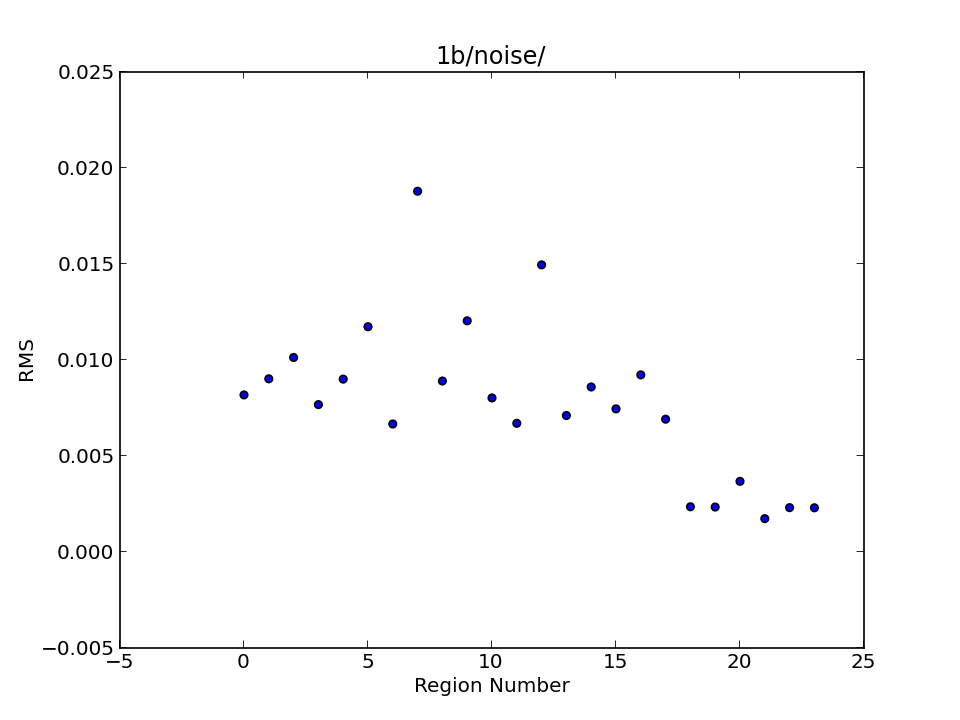
\includegraphics[width=.5\textwidth]{images/1b/noise/rms_over_time.png}
	\caption{RMS between the brightness values used to produce the synthetic curves and the brightness values recovered by the Amoeba Algorithm.}
	\label{rms12}
\end{figure}
\begin{figure}[h]
	\centering
	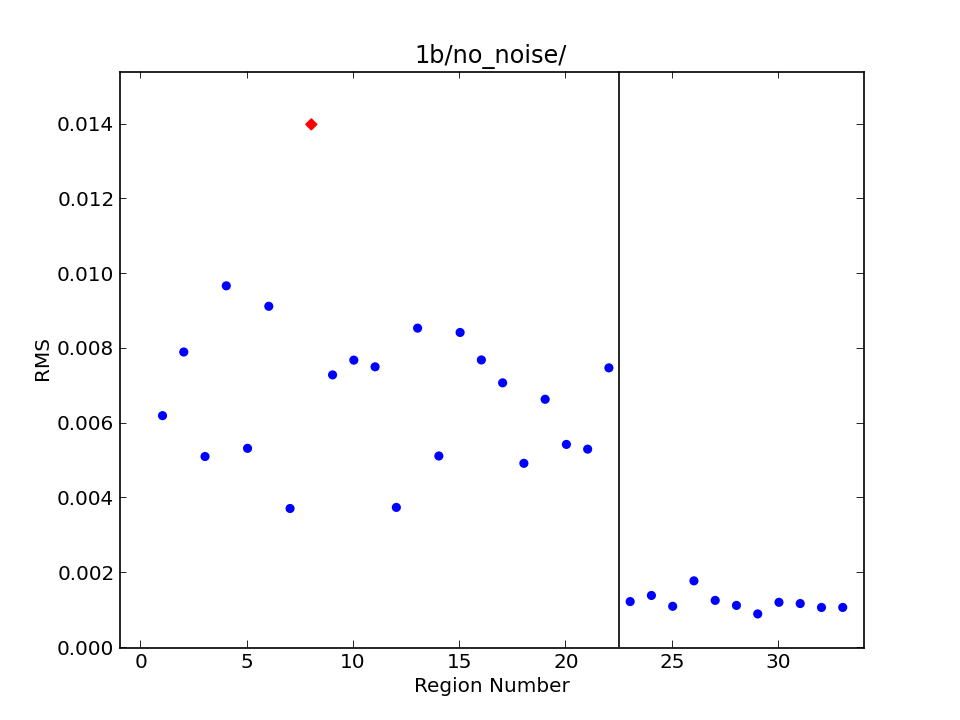
\includegraphics[width=.5\textwidth]{images/1b/no_noise/rms_over_time.png}
	\caption{RMS between the brightness values used to produce the synthetic curves and the brightness values recovered by the Amoeba Algorithm.}
	\label{rms}
\end{figure}

This particular set of images shows the brightness recovery for a synthetic light curve produced by darkening two stripe regions and two box regions and simulated 14th magnitude Gaussian noise. The code does a good job of recovering the brightness values for both boxes and stripes. The stripes, in general, are recovered more of the time, more precisely, and more accurately than the boxes. At any given window, one can usually believe a particular stripe measurement. The resulting stellar brightness map from this same set of recovered brightness values is shown in Figure~\ref{bright_map}.


%Figures for the text
%1b_1s
%3b_2s
%all_b_2s